{最小生成树是{一个有n个结点的连通图的生成树是原图的极小连通子图,且包含原图中的所有n个结点,并且有保持图连通的最少的边。}}

{最小生成树的总结:}

{性质1:使用不同的遍历图的方法,可以得到不同的生成树;从不同的顶点出发,也可能得到不同的生成树。}

{性质2:按照生成树的定义,n个顶点的连通网络的生成树有n个顶点、n-1条边。}

{性质3:构造最小生成树的准则:}

{①必须使用且仅使用该网络中的n-1条边来连接网络中的n个顶点;}

{②不能使用产生回路的边;}

{③各边上的权值的总和达到最小。}

{\textbf{2. 普里姆算法}}

{从连通网络N=\{V,E\}中的某一顶点u出发,选择与它关联的具有最小权值的边(u,v),将其顶点加入到生成树顶点集合U中。以后每一步从一个顶点在U中,而另一个顶点不在U中的各条边中选择权值最小的边(u,v),把它的顶点加入到集合U中。如此继续下去,直到网络中的所有顶点都加入到生成树顶点集合U中为止(读者可以用下图所示的例子实践一下,明白过程即可,一般考研试卷不直接考查代码实现)。}

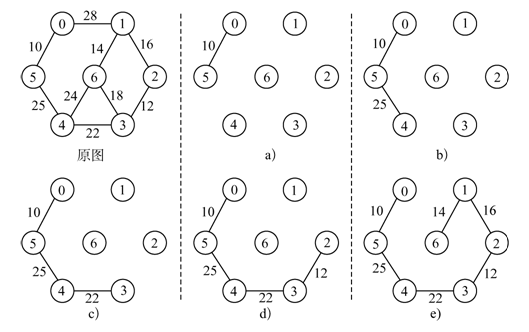
\includegraphics[width=3.70833in,height=2.32292in]{png-jpeg-pics/D43193B0360B43E38FBD1456AE03CDF3.png}

{总结:}

{(1)普里姆算法的复杂度为O(n\textsuperscript{2})。}

{(2){普里姆算法适用于稠密图}。}

% {\\
% }

{\textbf{2. 克鲁斯卡尔算法}}

{将下图中边按权值从小到大排序,然后从最小边开始扫描,并检测当前边是否为候选边(即是否该边的并入会构成回路),如不构成回路,则将该边并入当前生成树中,直到所有边都被检测完为止。(读者可以用如下图所示的例子实践一下,明白过程即可,一般考研试卷不直接考查代码实现)}

{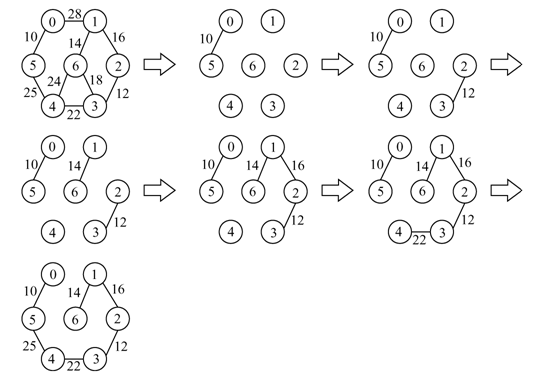
\includegraphics[width=3.70833in,height=2.59375in]{png-jpeg-pics/07BF7741A39C5FE66EBE18C782A6EC16.png}\\
\hspace*{0.333em}}

{总结:}

{(1)复杂度取决于排序算法。}

{(2)克鲁斯卡尔算法适用于稀疏图。}
